\documentclass[a4paper]{article}

\usepackage{a4wide}
\usepackage{tikz}
\usepackage{tikz-qtree}
\usepackage{amsmath,amssymb}

%\usetikzlibrary{automata,positioning,arrows,shapes,matrix}
\usetikzlibrary{automata}    % Styles 'state', 'initial', 'accepting'
\usetikzlibrary{positioning} % Function of ([right=of x])

% Global tikz settings
\tikzset{
semithick, % All lines semithick
>=stealth, % All arrows with stealth tick
my state/.style={draw,rectangle,rounded corners=2mm,minimum height=1.75em,minimum width=2em},
my accepting/.style={double,double distance=1pt,outer sep=0.9pt,semithick},
longer1/.style={shorten >=-0.425mm,shorten <=-0.5mm},
longer2/.style={shorten >=-0.7mm,shorten <=-0.8mm},
automaton/.style={
  every state/.style={my state},
  accepting/.style={my accepting},
  initial text=,
  every loop/.style={min distance=6mm,looseness=7},
  my below/.style={out=295,in=245},
  my above/.style={out=115,in=65},
},
my vdist/.code={\def\myvdist{#1}},
my vdist=1.2cm,
my hdist/.code={\def\myhdist{#1}},
my hdist=0.5cm,
tree/.style={
  every node/.style={draw,my state},
  acc/.style={my accepting},
  level distance=\myvdist,
  sibling distance=\myhdist,
},
tree example sets/.style={
  0/.style= {font={$\{q_0\}$}},
  1/.style= {font={$\{q_1\}$},acc},
  2/.style= {font={$\{q_2\}$}},
  02/.style={font={$\{q_0,q_2\}$}},
},
tree example no sets/.style={
  0/.style={font={$q_0$}},
  1/.style={font={$q_1$},acc},
  2/.style={font={$q_2$}},
},
dag/.style={
  acc/.style={my accepting},
  ghost/.style={draw=black!20,color=black!20},
  row sep={\myvdist,between origins},
  column sep=0.75cm
}
}

\newcommand{\automaton}{
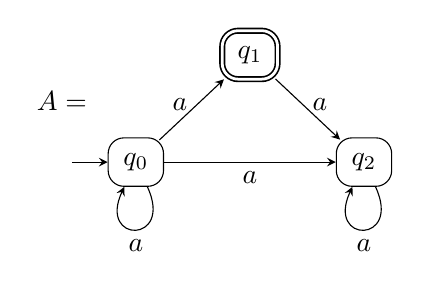
\begin{tikzpicture}[automaton,node distance=1cm]
\node[state,initial]   (0)                    {$q_0$};
\node[state,accepting] (1) [above right=of 0] {$q_1$};
\node[state]           (2) [below right=of 1] {$q_2$};

\path[->] (0) edge[my below,loop] node[below] {$a$} ()
              edge[longer1]        node[pos=0.3,above](m) {$a$} (1)
              edge                node[below] {$a$} (2)
          (1) edge[longer1]        node[pos=0.7,above] {$a$} (2)
          (2) edge[my below,loop] node[below] {$a$} ();

\node[draw=none,anchor=base,xshift=-1.5cm] at (m.base){$A=$};  
\end{tikzpicture}
}

\newcommand{\symbols}{
\begin{tikzpicture}[
level distance=\myvdist,
l/.style={pos=0.3,font={$a$}},
e/.style={draw=none}]
\Tree [ \edge[e] node[l]{}; [ \edge[e] node[l]{}; [ \edge[e] node[l]{}; [ \edge[e] node[l]{}; {} ] ] ] ]
\end{tikzpicture}
}

\begin{document}

\begin{figure}
\begin{center}
\automaton
\hfill
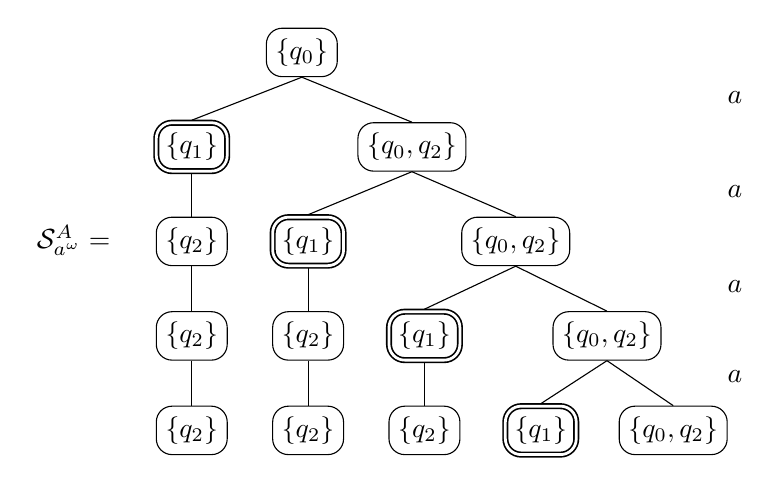
\begin{tikzpicture}[tree,tree example sets]
\Tree
[.\node[0]{}; [.\node[1]{};  [.\node[2](m){};  [.\node[2]{};  \node[2]{}; ] ] ]
              [.\node[02]{}; [.\node[1]{};  [.\node[2]{};  \node[2]{}; ] ]
                             [.\node[02]{}; [.\node[1]{};  \node[2]{}; ]
                                            [.\node[02]{}; \node[1]{};
                                                           \node[02]{}; ] ] ] ]
\node[draw=none,anchor=base,xshift=-1.5cm] at (m.base) {$\mathcal{S}^A_{a^\omega}=$};
\begin{scope}[every node/.style={draw=none,xshift=2.75cm}]
\Tree
[ \edge[draw=none] node[pos=.4]{$a$}; [ \edge[draw=none] node[pos=.4]{$a$}; [ \edge[draw=none] node[pos=.4]{$a$}; [ \edge[draw=none] node[pos=.4]{$a$}; {} ]  ] ] ]
\end{scope}
\end{tikzpicture}
%\symbols
\end{center}
\caption{Automaton $A$ and the first five levels of the split tree of the runs of $A$ on the word $a^\omega$.}
\end{figure}

\begin{figure}
\begin{center}

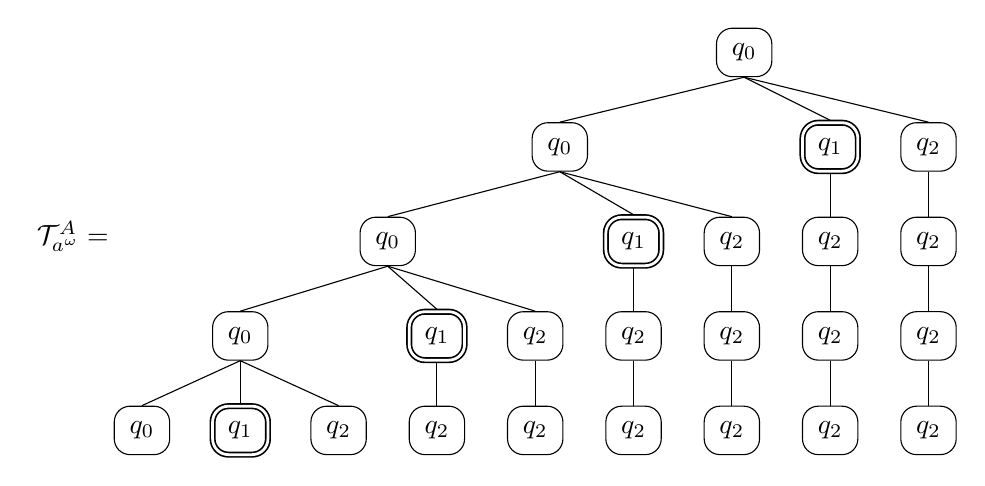
\begin{tikzpicture}[tree,tree example no sets]
\Tree
[.\node[0]{}; [.\node[0]{}; [.\node[0](m){}; [.\node[0]{};  \node[0]{};
                                                            \node[1]{};
                                                            \node[2]{}; ]
                                              [.\node[1]{}; \node[2]{}; ]
                                              [.\node[2]{}; \node[2]{}; ] ]
                            [.\node[1]{};     [.\node[2]{}; \node[2]{}; ] ]
                            [.\node[2]{};     [.\node[2]{}; \node[2]{}; ] ] ]
              [.\node[1]{}; [.\node[2]{};    [.\node[2]{};  \node[2]{}; ] ] ]
              [.\node[2]{}; [.\node[2]{};   [.\node[2]{};  \node[2]{}; ] ] ] ]

\node[draw=none,anchor=base,xshift=-4cm] at (m.base) {$\mathcal{T}^A_{a^\omega}=$};
% \begin{scope}[every node/.style={draw=none,xshift=2.75cm}]
% \Tree
% [ \edge[draw=none] node[pos=.4]{$a$}; [ \edge[draw=none] node[pos=.4]{$a$}; [ \edge[draw=none] node[pos=.4]{$a$}; [ \edge[draw=none] node[pos=.4]{$a$}; {} ]  ] ] ]
% \end{scope}
\end{tikzpicture}
\symbols
\end{center}
\caption{Automaton $A$ and the first five levels of the run tree of the runs of $A$ on the word $a^\omega$.}
\end{figure}

\begin{figure}
\begin{center}
\automaton
\hfil
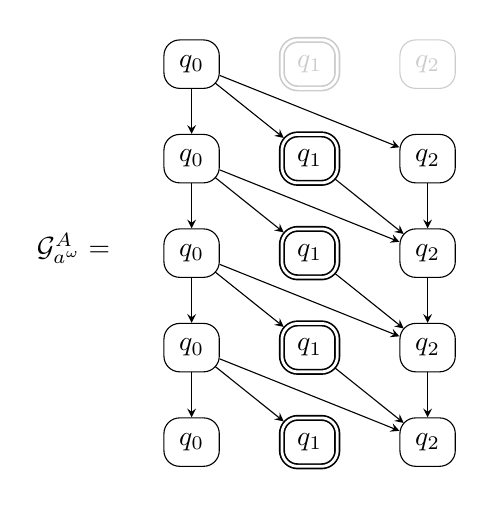
\begin{tikzpicture}[dag,tree example no sets]  
\matrix[every node/.style={my state}]{
  \node[0] (00) {}; & \node[1,ghost] (01) {}; & \node[2,ghost] (02) {}; \\
  \node[0] (10) {}; & \node[1] (11) {}; & \node[2] (12) {}; \\
  \node[0] (20) {}; & \node[1] (21) {}; & \node[2] (22) {}; \\
  \node[0] (30) {}; & \node[1] (31) {}; & \node[2] (32) {}; \\
  \node[0] (40) {}; & \node[1] (41) {}; & \node[2] (42) {}; \\
};
\path[->]
  (00) edge (10) edge[longer2] (11) edge (12)
  (10) edge (20) edge[longer2] (21) edge (22)
  (11) edge[longer2] (22)
  (12) edge (22)
  (20) edge (30) edge[longer2] (31) edge (32)
  (21) edge[longer2] (32)
  (22) edge (32)
  (30) edge (40) edge[longer2] (41) edge (42)
  (31) edge[longer2] (42)
  (32) edge (42);  
\node[anchor=base,xshift=-1.5cm] at (20.base) {$\mathcal{G}^A_{a^\omega}=$};      
\end{tikzpicture}
\symbols
\end{center}
\caption{Automaton $A$ and the first five levels of the run \textsc{dag} of the runs of $A$ on the word $a^\omega$.}
\end{figure}



\end{document}